\subsection{The Syntax of Encryption}
Some terms:
\begin{itemize}
    \item $M$: message space
    \item $C$: ciphertext space
    \item $K$: key space
    \item Three algorithms
    \begin{itemize}
        \item Key Generation: \textbf{Gen} is a \emph{probabilistic} algorithm that outputs a key $k \in K$ chosen according to some distribution.
        \item Encryption: \textbf{Enc} takes as input a key $k \in K$ and a message $m \in M$ and outputs a ciphertext $c \in C$.
        \item Decryption: \textbf{Dec} takes as input a key $k \in K$ and a ciphertext $c \in C$ and outputs a message $m \in M$.
    \end{itemize}
\end{itemize}

\subsection{Classical Ciphers}

\subsubsection{Caesar Cipher}
The Caesar cipher is one of the simplest and oldest encryption techniques, named after Julius Caesar, who used it to secure his communications. It works by shifting the letters of the alphabet by a fixed number of positions. For example, with a shift of 3, the letter ``A" becomes ``D", ``B" becomes ``E", and so on. To decrypt a message, the recipient simply shifts the letters back by the same number. Although it is easy to understand and implement, the Caesar cipher is considered insecure by modern standards, as there are only a limited number of possible shifts (25), making it vulnerable to brute force attacks.

\subsubsection{Shift Cipher}
A keyed variant of Caesar's cipher: the secret key can take value between 0 and 26. Each letter in the plaintext is shifted by a certain number of positions in the alphabet. The key difference is that the shift can vary, meaning the amount of movement of each letter can differ across the message. In a typical shift cipher, a number (the key) determines how far to shift each letter. Decryption requires shifting in the opposite direction by the same key. Like the Caesar cipher, the shift cipher is vulnerable to brute force attacks due to the limited number of possible shifts.

\[ c = m + k \mod 26 \]

Cryptanalysis of the shift cipher can be done using letter and bigram frequencies. This cipher is based on language, and language has structure. Thus it can be decrypted.  This approach leverages the fact that in natural languages, certain letters or combinations of letters appear more frequently than others. Example approach:
\begin{itemize}
    \item \textbf{Analyze the ciphertext}: Count the frequency of each letter in the encrypted message.
    \item \textbf{Compare with language statistics}: Match the observed frequencies with the known frequency distribution of letters in the target language (e.g., ``E'' is often the most frequent in English).
    \item \textbf{Make educated guesses}: Substitute frequently occurring ciphertext letters with likely plaintext letters.
    \item \textbf{Refine the substitution}: Use context, common words, and patterns to adjust and decode the message.
\end{itemize}

\subsubsection{Statistical Distance}
Used to evaluate the security of cryptographic systems by measuring how close an observed probability distribution (e.g., the distribution of ciphertexts) is to a desired distribution (usually uniform). Attacks can exploit patterns or non-uniformity in data. The goal is that a secure encryption scheme produces ciphertext that is statistically indistinguishable from random noise.

\[ \delta[X,Y] = \frac{1}{2}\sum_{u\in V} \left| \text{Pr}_{X \leftarrow D_1}[X = u]  - \text{Pr}_{Y \leftarrow D_2}[Y = u]  \right| \]

where $X, Y$ are random variables with distributions $D_1, D2$ respectively. \\

The statistical distance between the ciphertext distribution (produced by the encryption scheme) and the uniform distribution is measured. A smaller statistical distance implies stronger security, as it becomes harder for an attacker to distinguish between encrypted data and random noise.

\subsubsection{Substitution Cipher}
Each letter (or symbol) in the plaintext is replaced with another letter or symbol according to a specific rule or mapping. The mapping defines the ``key" for the cipher, and the process is reversible if the recipient knows the key.
The key space consists of all bijections, or permutations ($26! \approx 2^{88}$ for English alphabet). But using letter frequencies, the cipher can be easily solved. \\

\textbf{Example:}
\begin{itemize}
    \item Plaintext: \texttt{HELLO}
    
    \item Cipher Key:
    \[
    \text{A} \rightarrow \text{Q}, \, \text{B} \rightarrow \text{W}, \, \text{C} \rightarrow \text{E}, \, \ldots, \, \text{Z} \rightarrow \text{P}
    \]

    \item Key mapping:
        \begin{itemize}
            \item Plain alphabet: \texttt{ABCDEFGHIJKLMNOPQRSTUVWXYZ}
            \item Cipher alphabet: \texttt{QWERTYUIOPASDFGHJKLZXCVBNM}
        \end{itemize}
    
    \item Ciphertext: \texttt{XUBBE}
\end{itemize}


\textbf{Types of Substitution Ciphers}:
    \begin{itemize}
        \item \emph{Mono-alphabetic}: Uses a single mapping for the entire message (e.g., Caesar cipher).
        \item \emph{Poly-alphabetic}: Uses multiple mappings that change throughout the message for added complexity.
    \end{itemize}

\subsubsection{Vigenère Cipher}
Also called a poly-alphabetic substitution cipher: encrypt each letter with a dfferent alphabet. Use a keyword to shift letters in the plaintext. Unlike the Caesar cipher, where each letter is shifted by a constant number, the Vigenère cipher uses a series of shifts based on the letters of a keyword. This makes it more secure than simple substitution ciphers, as the pattern of shifts changes across the message.  Still, cryptanalysis is easy.

\begin{defn}
    \textbf{Kasiski Test:} Find the occurence of the repeated sequences and use $\gcd$ to determine the key length.
\end{defn}

The plaintext is encrypted by shifting each letter by the number of positions specified by the corresponding letter in the keyword. If the keyword is shorter than the plaintext, it is repeated until it matches the length of the plaintext.\\

\textbf{Example:} \begin{itemize}
    \item Plaintext: \texttt{HELLO}
    
    \item Keyword: \texttt{KEY}
    
    \item Repeat the keyword to match the length of the plaintext: \texttt{KEYKE}
    
    \item Shift each letter in the plaintext by the corresponding letter in the keyword:
    \begin{itemize}
        \item \texttt{H} (shift by \texttt{K}, which is 10) $\rightarrow$ \texttt{R}
        \item \texttt{E} (shift by \texttt{E}, which is 4) $\rightarrow$ \texttt{I}
        \item \texttt{L} (shift by \texttt{Y}, which is 24) $\rightarrow$ \texttt{J}
        \item \texttt{L} (shift by \texttt{K}, which is 10) $\rightarrow$ \texttt{V}
        \item \texttt{O} (shift by \texttt{E}, which is 4) $\rightarrow$ \texttt{S}
    \end{itemize}
    
    \item Ciphertext: \texttt{RIJVS}
\end{itemize}

\subsubsection{Permutation Cipher}
The \emph{positions} of the characters in the plaintext are rearranged according to a specific permutation (a predetermined key) rather than \emph{replacing} characters with other symbols. The basic idea is that the order of the characters is shuffled, but no new symbols are introduced. \\

\begin{figure}[h!]
    \centering
    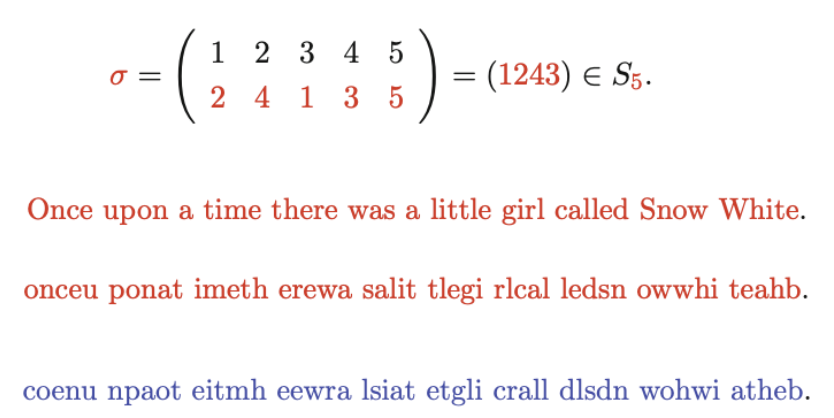
\includegraphics[width=0.5\linewidth]{img/permcipher.png}
    \caption{Permutation Cipher}
\end{figure}

The key is a sequence of numbers that indicates the new positions of each character in the plaintext. Here, $(1243) \in S_5$, meaning; position 1 goes to position 2, position 2 goes to position 4, and so on. The key space is $|S_n| = n!$. \\

Key take aways: all historical, classical systems are broken. They rely on substituion and permutation. Designing secure ciphers is hard. 